\documentclass{article}
%\usepackage{pdftricks}
%\usepackage{pst-all}
\usepackage{pstricks}
% if you use the following package straight latex running (not via pdflatex), will not work...
%\usepackage{pst-pdf}
%\usepackage{auto-pst-pdf}
\usepackage{tikz}
\usepackage{amssymb,amsmath,color,thumbpdf,html,hyperref}
%%\usepackage{pst-barcode,pstricks-add}

\title{Riddles}
\author{Mark Veltzer}
\date{\today}

\begin{document}

\maketitle

\tableofcontents

\section{Rational points on a circle}

%\subsection{Question}

Could there be a circle on the plane where only one point has rational co-ordinates? A point has rational co-ordinates if $x,y\in\mathbb{Q}$. What about a sphere? Are there circles with more than one rational point? Are there circles with infinite rational points? Can you find a circle with exactly $n$ rational points on it for each $n\in\mathbb{N}$?

\subsection{Solution}

Yes, there could. Consider the circle: $(x-r)^2+y^2=r^2$ for some irrational $r$.
$(0,0)$ is a point on this circle and is rational. But from the equation it follows
that: $x^2-2xr+r^2+y^2=r^2$ or $x^2+y^2=2xr$ or $r=(x^2+y^2)/2x$. If there
was a rational solution to this equation where $x\ne0$ then it would follow that
$r$ is rational since it is the result of multiplication, division, addition and subtration
of rational numbers and this is a contradiction. This means this equation can only
have rational solutions for $x=0$. If $x=0$ then $r^2+y^2=r^2$ and so $y=0$ and so
$(0,0)$ is the only such solution.

Same solution applies to a sphere: $(x-r)^2+y^2+z^2=r^2$ for some irrational $r$.
In this case: $r=(x^2+y^2+z^2)/2x$. Which means that for $x\ne0$ any rational soultion would imply a rational $r$.
$(0,0,0)$ is therefor the only rational solution.

Yes, there are circles with more than one rational point. Take $x^2+y^2=2$ which is the circle whose
center is at $(0,0)$ and whose radius is $\sqrt{2}$. The points $(1,1),(-1,1),(1,-1),(-1,-1)$ are four rational
points which are on this circle.

Yes, there are circles with infinite rational points.

\section{Always lead in election (combinatorics)}

%\subsection{Question}

%id=elections (for out of source references to this riddle)

An election was voted a perfect tie (even number of electors) and was decided by way of putting
all the votes into a hat, mixing them uniformly and counting them one by one. What is the chance
that one of the candidates was leading during the entire counting process?

\subsection{Solution}

The question could be rephrased as how many graphs that go either one step up or one step down (lets call those binary graphs) do not go down below zero out of the set of all graphs that go from zero to zero. At first lets note that in the following solution $n$ is even and so there is no problem with $n/2$. A first observation is that the set of all graphs going from 0 to 0 in $n$ steps is ${n \choose n/2}$.

Let's try to count the graphs that tip below 0. Every graph that tips below 0 will reach -1 at one or more points. Lets find the first place where the graph reaches -1. From that point on the graph climbs one more than it descends since it finally reaches 0. Lets flip it from that point on - meaning switch every climb with descent and every descent with a climb. Now the graph descends one more than it climbs and since it starts from that point at height -1 then it now reaches a height -2 at $n$ instead of the original 0.

The main proposition is that \emph{every} graph which travels from 0 to -2 correspons with a \emph{1-1 correspondance} to graphs that travel from 0 to 0 and reach -1 at some point (convince yourself
of this).

If this is so then the number of graphs that go from 0 to -2 is ${n \choose n/2+1}$ since we need to
choose points at which the graph will go down and we have $n/2+1$ descends. If so then the number of
graphs that do not reach -1 is:

${n \choose n/2} - {n \choose n/2+1} = \frac{(n)!}{(n/2+1)!(n/2)!} = \frac{1}{n/2+1}{n \choose n/2}$.

And now back to the original question "What is the chance that one of the candidates was leading the whole time?". Well divide the latter result with the former and we get:

$\frac{1}{n/2+1}{n \choose n/2} / {n \choose n/2} = \frac{1}{n/2+1}$

The result is all about \htmladdnormallink{Catalan numbers}{http://en.wikipedia.org/wiki/Catalan_number}
and \htmladdnormallink{Bertrand's ballot theorem}{http://en.wikipedia.org/wiki/Bertrand\%27s_ballot_theorem}.

\section{Four Coke bottles on a table}

Arrange four Coke bottles on a table so that the distances between each pair of caps will be the same. Assume that
you can make a Coke bottle stand on it's head (this is a pretty strong hint!, maybe I should remove it ?!?).

\subsection{Solution}

There are two solutions:

The first solution is to put the bottles in a square where each the side of the square is the length of the bottle. Bottles
next to each other will stand \emph{in reverse} (if the first is on it's head the the second will stand straight).
The distance between each two bottles will be $\sqrt{2l^2}$.

% Sketch output, version 0.3 (build 7d, Wed May 2 06:36:52 2012)
% Output language: PGF/TikZ,LaTeX
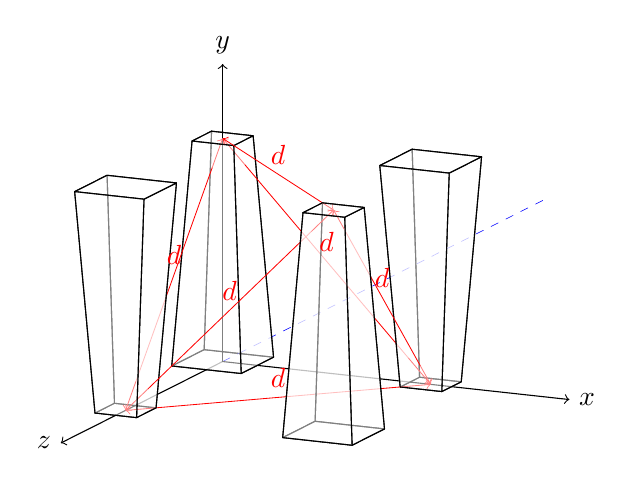
\begin{tikzpicture}[line join=round]
\draw[arrows=-](-2.055,-1.034)--(-2.261,-1.138);
\filldraw[fill opacity=0.5,fill=white](-2.29,-.883)--(-2.701,-1.09)--(-1.82,-1.186)--(-1.409,-.979)--cycle;
\draw[line width=.2pt,draw=blue,dashed](-1.85,-.931)--(2.055,1.034);
\filldraw[fill opacity=0.5,fill=white](-1.409,-.979)--(-2.29,-.883)--(-2.196,1.891)--(-1.668,1.833)--cycle;
\filldraw[fill opacity=0.5,fill=white](-2.29,-.883)--(-2.701,-1.09)--(-2.443,1.767)--(-2.196,1.891)--cycle;
\draw[line width=.2pt,draw=blue,dashed](-2.055,-1.034)--(-1.85,-.931);
\draw[arrows=-](-2.055,-1.034)--(-1.615,-1.083);
\draw[line width=.3pt,arrows=<-,draw=red](-2.055,1.8)--(-1.772,1.465);
\filldraw[fill opacity=0.5,fill=white](-1.82,-1.186)--(-1.409,-.979)--(-1.668,1.833)--(-1.914,1.709)--cycle;
\draw[arrows=-](-2.055,-1.034)--(-2.055,1.8);
\filldraw[fill opacity=0.5,fill=white](.975,-1.291)--(.728,-1.415)--(.2,-1.357)--(.446,-1.233)--cycle;
\draw[arrows=-](-1.615,-1.083)--(.323,-1.295);
\draw[line width=.3pt,arrows=->,draw=red](-2.187,1.43)--(-2.055,1.8);
\filldraw[fill opacity=0.5,fill=white](-2.701,-1.09)--(-1.82,-1.186)--(-1.914,1.709)--(-2.443,1.767)--cycle;
\filldraw[fill opacity=0.5,fill=white](-2.196,1.891)--(-2.443,1.767)--(-1.914,1.709)--(-1.668,1.833)--cycle;
\draw[arrows=-](-2.261,-1.138)--(-3.165,-1.593);
\draw[arrows=->](-2.055,1.8)--(-2.055,2.745);
\draw[line width=.3pt,arrows=<-,draw=red](-2.055,1.8)--(-1.914,1.709);
\draw[line width=.3pt,arrows=-,draw=red](-1.772,1.465)--(.304,-.989);
\filldraw[fill opacity=0.5,fill=white](-.059,1.455)--(.352,1.662)--(.446,-1.233)--(.2,-1.357)--cycle;
\filldraw[fill opacity=0.5,fill=white](.352,1.662)--(1.233,1.566)--(.975,-1.291)--(.446,-1.233)--cycle;
\draw[line width=.3pt,arrows=-,draw=red](-3.156,-1.285)--(-2.187,1.43);
\draw[line width=.3pt,arrows=-,draw=red](-1.914,1.709)--(-.787,.981);
\draw[arrows=-](.323,-1.295)--(.851,-1.353);
\filldraw[fill opacity=0.5,fill=white](1.233,1.566)--(.822,1.359)--(.728,-1.415)--(.975,-1.291)--cycle;
\draw[line width=.3pt,arrows=->,draw=red](.304,-.989)--(.587,-1.324);
\draw[line width=.3pt,arrows=<-,draw=red](.587,-1.324)--(.2,-1.357);
\draw[line width=.3pt,arrows=<-,draw=red](.587,-1.324)--(.455,-1.087);
\filldraw[fill opacity=0.5,fill=white](1.233,1.566)--(.822,1.359)--(-.059,1.455)--(.352,1.662)--cycle;
\draw[arrows=->](.851,-1.353)--(2.349,-1.517);
\filldraw[fill opacity=0.5,fill=white](.822,1.359)--(-.059,1.455)--(.2,-1.357)--(.728,-1.415)--cycle;
\filldraw[fill opacity=0.5,fill=white](-2.901,-1.622)--(-3.148,-1.746)--(-3.676,-1.688)--(-3.429,-1.564)--cycle;
\draw[line width=.3pt,arrows=-,draw=red](.2,-1.357)--(-2.901,-1.622);
\draw[line width=.3pt,arrows=-,draw=red](.455,-1.087)--(-.514,.652);
\filldraw[fill opacity=0.5,fill=white](-3.523,1.331)--(-2.642,1.234)--(-2.901,-1.622)--(-3.429,-1.564)--cycle;
\filldraw[fill opacity=0.5,fill=white](-3.934,1.124)--(-3.523,1.331)--(-3.429,-1.564)--(-3.676,-1.688)--cycle;
\draw[arrows=-](-3.165,-1.593)--(-3.412,-1.717);
\draw[line width=.3pt,arrows=<-,draw=red](-3.288,-1.655)--(-3.156,-1.285);
\draw[line width=.3pt,arrows=->,draw=red](-2.901,-1.622)--(-3.288,-1.655);
\draw[line width=.3pt,arrows=->,draw=red](-3.005,-1.383)--(-3.288,-1.655);
\filldraw[fill opacity=0.5,fill=white](-2.642,1.234)--(-3.054,1.028)--(-3.148,-1.746)--(-2.901,-1.622)--cycle;
\filldraw[fill opacity=0.5,fill=white](-2.642,1.234)--(-3.054,1.028)--(-3.934,1.124)--(-3.523,1.331)--cycle;
\filldraw[fill opacity=0.5,fill=white](-3.054,1.028)--(-3.934,1.124)--(-3.676,-1.688)--(-3.148,-1.746)--cycle;
\filldraw[fill opacity=0.5,fill=white](0,-1.89)--(-.881,-1.793)--(-.787,.981)--(-.258,.923)--cycle;
\draw[line width=.3pt,arrows=-,draw=red](-.929,.617)--(-3.005,-1.383);
\draw[arrows=->](-3.412,-1.717)--(-4.111,-2.069);
\filldraw[fill opacity=0.5,fill=white](-.881,-1.793)--(-1.292,-2)--(-1.034,.857)--(-.787,.981)--cycle;
\filldraw[fill opacity=0.5,fill=white](-.881,-1.793)--(-1.292,-2)--(-.411,-2.097)--(0,-1.89)--cycle;
\filldraw[fill opacity=0.5,fill=white](-.411,-2.097)--(0,-1.89)--(-.258,.923)--(-.505,.799)--cycle;
\draw[line width=.3pt,arrows=->,draw=red](-.514,.652)--(-.646,.89);
\draw[line width=.3pt,arrows=<-,draw=red](-.646,.89)--(-.929,.617);
\filldraw[fill opacity=0.5,fill=white](-1.292,-2)--(-.411,-2.097)--(-.505,.799)--(-1.034,.857)--cycle;
\draw[line width=.3pt,arrows=->,draw=red](-.787,.981)--(-.646,.89);
\filldraw[fill opacity=0.5,fill=white](-.787,.981)--(-1.034,.857)--(-.505,.799)--(-.258,.923)--cycle;
\node[right] at (2.349,-1.517) {$x$};\node[above] at (-2.055,2.745) {$y$};\node[left] at (-4.111,-2.069) {$z$};\node[above,color=red] at (-1.351,1.345) {$d$};\node[above,color=red] at (-1.351,-1.49) {$d$};\node[above,color=red] at (-.734,.238) {$d$};\node[above,color=red] at (-.029,-.217) {$d$};\node[above,color=red] at (-1.967,-.383) {$d$};\node[above,color=red] at (-2.672,.072) {$d$};\end{tikzpicture}% End sketch output


The second solution is to put three bottles on the vertices of an even sided triangle standing one way. The fourth will be placed
in the middle of the triangle and will be standing reversed to the others. The problem is here is to calculate the side of the triangle (TODO).
Lets call the length of the triangle $d$. Then the height of the base triagle.

% Sketch output, version 0.3 (build 7d, Wed May 2 06:36:52 2012)
% Output language: PGF/TikZ,LaTeX
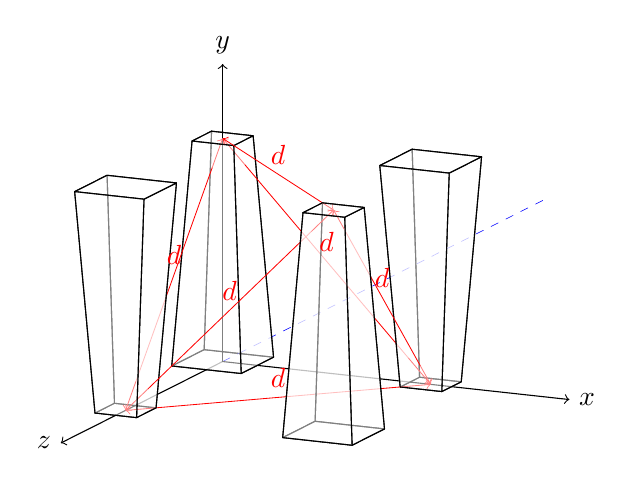
\begin{tikzpicture}[line join=round]
\draw[arrows=-](-2.055,-1.034)--(-2.261,-1.138);
\filldraw[fill opacity=0.5,fill=white](-2.29,-.883)--(-2.701,-1.09)--(-1.82,-1.186)--(-1.409,-.979)--cycle;
\draw[line width=.2pt,draw=blue,dashed](-1.85,-.931)--(2.055,1.034);
\filldraw[fill opacity=0.5,fill=white](-1.409,-.979)--(-2.29,-.883)--(-2.196,1.891)--(-1.668,1.833)--cycle;
\filldraw[fill opacity=0.5,fill=white](-2.29,-.883)--(-2.701,-1.09)--(-2.443,1.767)--(-2.196,1.891)--cycle;
\draw[line width=.2pt,draw=blue,dashed](-2.055,-1.034)--(-1.85,-.931);
\draw[arrows=-](-2.055,-1.034)--(-1.615,-1.083);
\draw[line width=.3pt,arrows=<-,draw=red](-2.055,1.8)--(-1.772,1.465);
\filldraw[fill opacity=0.5,fill=white](-1.82,-1.186)--(-1.409,-.979)--(-1.668,1.833)--(-1.914,1.709)--cycle;
\draw[arrows=-](-2.055,-1.034)--(-2.055,1.8);
\filldraw[fill opacity=0.5,fill=white](.975,-1.291)--(.728,-1.415)--(.2,-1.357)--(.446,-1.233)--cycle;
\draw[arrows=-](-1.615,-1.083)--(.323,-1.295);
\draw[line width=.3pt,arrows=->,draw=red](-2.187,1.43)--(-2.055,1.8);
\filldraw[fill opacity=0.5,fill=white](-2.701,-1.09)--(-1.82,-1.186)--(-1.914,1.709)--(-2.443,1.767)--cycle;
\filldraw[fill opacity=0.5,fill=white](-2.196,1.891)--(-2.443,1.767)--(-1.914,1.709)--(-1.668,1.833)--cycle;
\draw[arrows=-](-2.261,-1.138)--(-3.165,-1.593);
\draw[arrows=->](-2.055,1.8)--(-2.055,2.745);
\draw[line width=.3pt,arrows=<-,draw=red](-2.055,1.8)--(-1.914,1.709);
\draw[line width=.3pt,arrows=-,draw=red](-1.772,1.465)--(.304,-.989);
\filldraw[fill opacity=0.5,fill=white](-.059,1.455)--(.352,1.662)--(.446,-1.233)--(.2,-1.357)--cycle;
\filldraw[fill opacity=0.5,fill=white](.352,1.662)--(1.233,1.566)--(.975,-1.291)--(.446,-1.233)--cycle;
\draw[line width=.3pt,arrows=-,draw=red](-3.156,-1.285)--(-2.187,1.43);
\draw[line width=.3pt,arrows=-,draw=red](-1.914,1.709)--(-.787,.981);
\draw[arrows=-](.323,-1.295)--(.851,-1.353);
\filldraw[fill opacity=0.5,fill=white](1.233,1.566)--(.822,1.359)--(.728,-1.415)--(.975,-1.291)--cycle;
\draw[line width=.3pt,arrows=->,draw=red](.304,-.989)--(.587,-1.324);
\draw[line width=.3pt,arrows=<-,draw=red](.587,-1.324)--(.2,-1.357);
\draw[line width=.3pt,arrows=<-,draw=red](.587,-1.324)--(.455,-1.087);
\filldraw[fill opacity=0.5,fill=white](1.233,1.566)--(.822,1.359)--(-.059,1.455)--(.352,1.662)--cycle;
\draw[arrows=->](.851,-1.353)--(2.349,-1.517);
\filldraw[fill opacity=0.5,fill=white](.822,1.359)--(-.059,1.455)--(.2,-1.357)--(.728,-1.415)--cycle;
\filldraw[fill opacity=0.5,fill=white](-2.901,-1.622)--(-3.148,-1.746)--(-3.676,-1.688)--(-3.429,-1.564)--cycle;
\draw[line width=.3pt,arrows=-,draw=red](.2,-1.357)--(-2.901,-1.622);
\draw[line width=.3pt,arrows=-,draw=red](.455,-1.087)--(-.514,.652);
\filldraw[fill opacity=0.5,fill=white](-3.523,1.331)--(-2.642,1.234)--(-2.901,-1.622)--(-3.429,-1.564)--cycle;
\filldraw[fill opacity=0.5,fill=white](-3.934,1.124)--(-3.523,1.331)--(-3.429,-1.564)--(-3.676,-1.688)--cycle;
\draw[arrows=-](-3.165,-1.593)--(-3.412,-1.717);
\draw[line width=.3pt,arrows=<-,draw=red](-3.288,-1.655)--(-3.156,-1.285);
\draw[line width=.3pt,arrows=->,draw=red](-2.901,-1.622)--(-3.288,-1.655);
\draw[line width=.3pt,arrows=->,draw=red](-3.005,-1.383)--(-3.288,-1.655);
\filldraw[fill opacity=0.5,fill=white](-2.642,1.234)--(-3.054,1.028)--(-3.148,-1.746)--(-2.901,-1.622)--cycle;
\filldraw[fill opacity=0.5,fill=white](-2.642,1.234)--(-3.054,1.028)--(-3.934,1.124)--(-3.523,1.331)--cycle;
\filldraw[fill opacity=0.5,fill=white](-3.054,1.028)--(-3.934,1.124)--(-3.676,-1.688)--(-3.148,-1.746)--cycle;
\filldraw[fill opacity=0.5,fill=white](0,-1.89)--(-.881,-1.793)--(-.787,.981)--(-.258,.923)--cycle;
\draw[line width=.3pt,arrows=-,draw=red](-.929,.617)--(-3.005,-1.383);
\draw[arrows=->](-3.412,-1.717)--(-4.111,-2.069);
\filldraw[fill opacity=0.5,fill=white](-.881,-1.793)--(-1.292,-2)--(-1.034,.857)--(-.787,.981)--cycle;
\filldraw[fill opacity=0.5,fill=white](-.881,-1.793)--(-1.292,-2)--(-.411,-2.097)--(0,-1.89)--cycle;
\filldraw[fill opacity=0.5,fill=white](-.411,-2.097)--(0,-1.89)--(-.258,.923)--(-.505,.799)--cycle;
\draw[line width=.3pt,arrows=->,draw=red](-.514,.652)--(-.646,.89);
\draw[line width=.3pt,arrows=<-,draw=red](-.646,.89)--(-.929,.617);
\filldraw[fill opacity=0.5,fill=white](-1.292,-2)--(-.411,-2.097)--(-.505,.799)--(-1.034,.857)--cycle;
\draw[line width=.3pt,arrows=->,draw=red](-.787,.981)--(-.646,.89);
\filldraw[fill opacity=0.5,fill=white](-.787,.981)--(-1.034,.857)--(-.505,.799)--(-.258,.923)--cycle;
\node[right] at (2.349,-1.517) {$x$};\node[above] at (-2.055,2.745) {$y$};\node[left] at (-4.111,-2.069) {$z$};\node[above,color=red] at (-1.351,1.345) {$d$};\node[above,color=red] at (-1.351,-1.49) {$d$};\node[above,color=red] at (-.734,.238) {$d$};\node[above,color=red] at (-.029,-.217) {$d$};\node[above,color=red] at (-1.967,-.383) {$d$};\node[above,color=red] at (-2.672,.072) {$d$};\end{tikzpicture}% End sketch output


\label{end}\end{document}
